\documentclass[alpha-refs]{wiley-article}

\usepackage[binary-units]{siunitx}
\usepackage{bm,bbm}
\usepackage{booktabs}
\usepackage{subfig}
\usepackage{float}
\usepackage{rotating}
\graphicspath{{./Figures/}}
\usepackage[linesnumbered,lined,boxed]{algorithm2e}
\makeatletter
\renewcommand{\@algocf@capt@plain}{above}% formerly {bottom}
\makeatother
\usepackage{undertilde}
\usepackage{tcolorbox}
\usepackage{todonotes}
\usepackage{comment}   

\begin{document}
\title{Manuscript ID ISR-OA-160-20}

\author{Eduarda T.\ C.\ Chagas, Marcelo Queiroz-Oliveira, Osvaldo A.\ Rosso, Heitor S.\ Ramos, Cristopher G.\ S. Freitas, and Alejandro C.\ Frery}

\papertype{Response Letter}
\maketitle

\section{Co-Editor-in-Chief Requirements}

\vskip3em\begin{tcolorbox}[colback=red!5!white,colframe=red!75!black,title=Comment \#1]
The editor has recommended a major revision, and I am inclined to agree. 
In particular, I would like to see a strong review component tied in with what you propose, and also a comparison of where your method stands in the literature. 
Substantiating the advantages through theory or simulation studies would be helpful as well. 
Please keep in mind that this is a review journal and that the paper must be accessible to more than the technical experts in the area.
\end{tcolorbox}

We wholeheartedly agree.
Our initial version did not make a clear statement of the article's nature.
In order to improve this issue, we have introduced two changes.
The first is a new title, namely
\begin{quote}
Time Series Analysis with Bandt \& Pompe Symbolization and a Test for White Noise in the Entropy-Complexity Plane
\end{quote}
Second, we now state at the beginning of the Abstract that
\begin{quote}
	This article serves two purposes.
	Firstly, it surveys the \citeauthor{PermutationEntropyBandtPompe} methodology for the statistical community, stressing topics that are open for research.
	Secondly, it contributes towards a better understanding of the statistical properties of that approach for time series analysis.
\end{quote}

We also updated the following paragraph from the Introduction:
\begin{quote}
	The \num{2,160} citations received by the seminal paper appeared in \num{780} venues indexed by the Web of Science.
	Among them, the journals belong to \num{127} categories, spanning from Multidisciplinary Physics (\SI{24}{\percent} of the publications) to Zoology (only one of the of citing articles).
	There are \num{22} citing articles from journals that belong to the Statistics \& Probability category.
	Five of these articles appeared in \textit{Stochastic Environmental Research and Risk Assessment}, 
	two in the \textit{Journal of Time Series Analysis} and in 
	\textit{Theory and Applications of Time Series Analysis},
	and each of the remaining ten appeared in a different journal.
	Most of these articles relate successful applications of the Bandt and Pompe methodology, except \cite{OrdinalPatternProbabilities} that obtained the sample entropy's properties under zero-mean Gaussian processes.
	It is also noteworthy that, in this category of publications, \cite{DistributionsofOrderPatternsofIntervalMaps} provided a formal and more general proof of the structure of the boundary of the $H\times C$ manifold than that obtained by \cite{martin2006generalized}.
	The lack of attention that the Bandt and Pompe approach has received by the Probability \& Statistics community confirms that it is a fertile research avenue waiting to explore.
\end{quote}

We hope these changes, which reflect our initial idea, make a clear point that this a contribution for the statistical community.

We have made other changes to improve the manuscript readability and conciseness.
For instance, we now provide explicit expressions for the normalized disequilibrium.
In particular, as detailed below, we now illustrate the need of using the complexity.

\section{Reviewer \#1}

\vskip3em\begin{tcolorbox}[colback=red!5!white,colframe=red!75!black,title=Comment \#1]
In this paper the authors propose a quite elaborate method to test whether a discrete-time analog signal is white noise by locating it in the entropy-complexity plane (ECP). The description is didactic, detailed and well-written. However, I missed the rationale of using the ECP. I mean, what can be done in this way that cannot be done with the entropy alone? After all, entropy (horizontal axis of the ECP) is a measure of (pseudo-)randomness. For white noise, the normalized (permutation) entropy is 1, hence complexity is automatically 0 (see the definition domain of the ECP in Figures 2, 4 and 5). In other words, why use two measures that are not independent (since entropy sets the range of complexity), instead of only one (the entropy in this case)? So, unless the authors convincingly rebut this point, I cannot recommend the publication of this paper in ISR.
\end{tcolorbox}

In fact, an infinitely large sample of white noise will produce a perfectly flat histogram of patterns which, in turn, becomes the point $(1,0)\in H\times C$.
Nevertheless, the finite sample size properties are almost completely unknown, and starting their study is one of the purposes of this paper.

\addtocounter{section}{2}
\addtocounter{subsection}{1}
\addtocounter{subsubsection}{1}
\addtocounter{figure}{11}
The reviewer rises a very relevant question: is the Statistical Complexity needed?
Several researchers have addressed this question, and the unanimous answer is yes, it is needed.
The discussion has been limited to the Physics literature, most markedly after the work by \citet{SimpleMeasureforComplexity} and the subsequent discussion \citep{CommentIonSimpleMeasureforComplexity,CommentIIonSimpleMeasureforComplexity} and rejoinder \citep{ReplytoCommentsonSimpleMeasureforComplexity} papers.

Going further in this direction would require introducing several concepts which may seem unfamiliar to this journal's readership.
Nevertheless, being an relevant point, we opted for illustrating the need of both descriptors, entropy and complexity, with an example in the discussion of the test power.

We split the power subsection in two, and added another study which illustrates the need of considering the complexity:
\begin{quote}
	\subsubsection{$H_1$: Patch of Deterministic Function}
	
	Consider the times series of length $T$ comprised of $T-[c100]$ white noise observations $x_1,x_2,\dots, x_{T-[c100]}$ followed by the signal $y_{T-[c100]+1}, y_{T-[c100]+2}, \dots, y_T$, in which $0\leq c \ll 1$ is the percentage of contamination.
	We will verify the behavior of our test for the case $T=1000$, and $y_t$ an increasing function on $t$.
	Fig.~\ref{Fig:PointsPatchedIncreasingFunction} shows the effect of such a contamination on the white noise time series whose point in the $H\times C$ plane appears in black.
	The Figure also shows the confidence region at \SI{99}{\percent}.
	
	\begin{figure}[hbt]
		\centering
		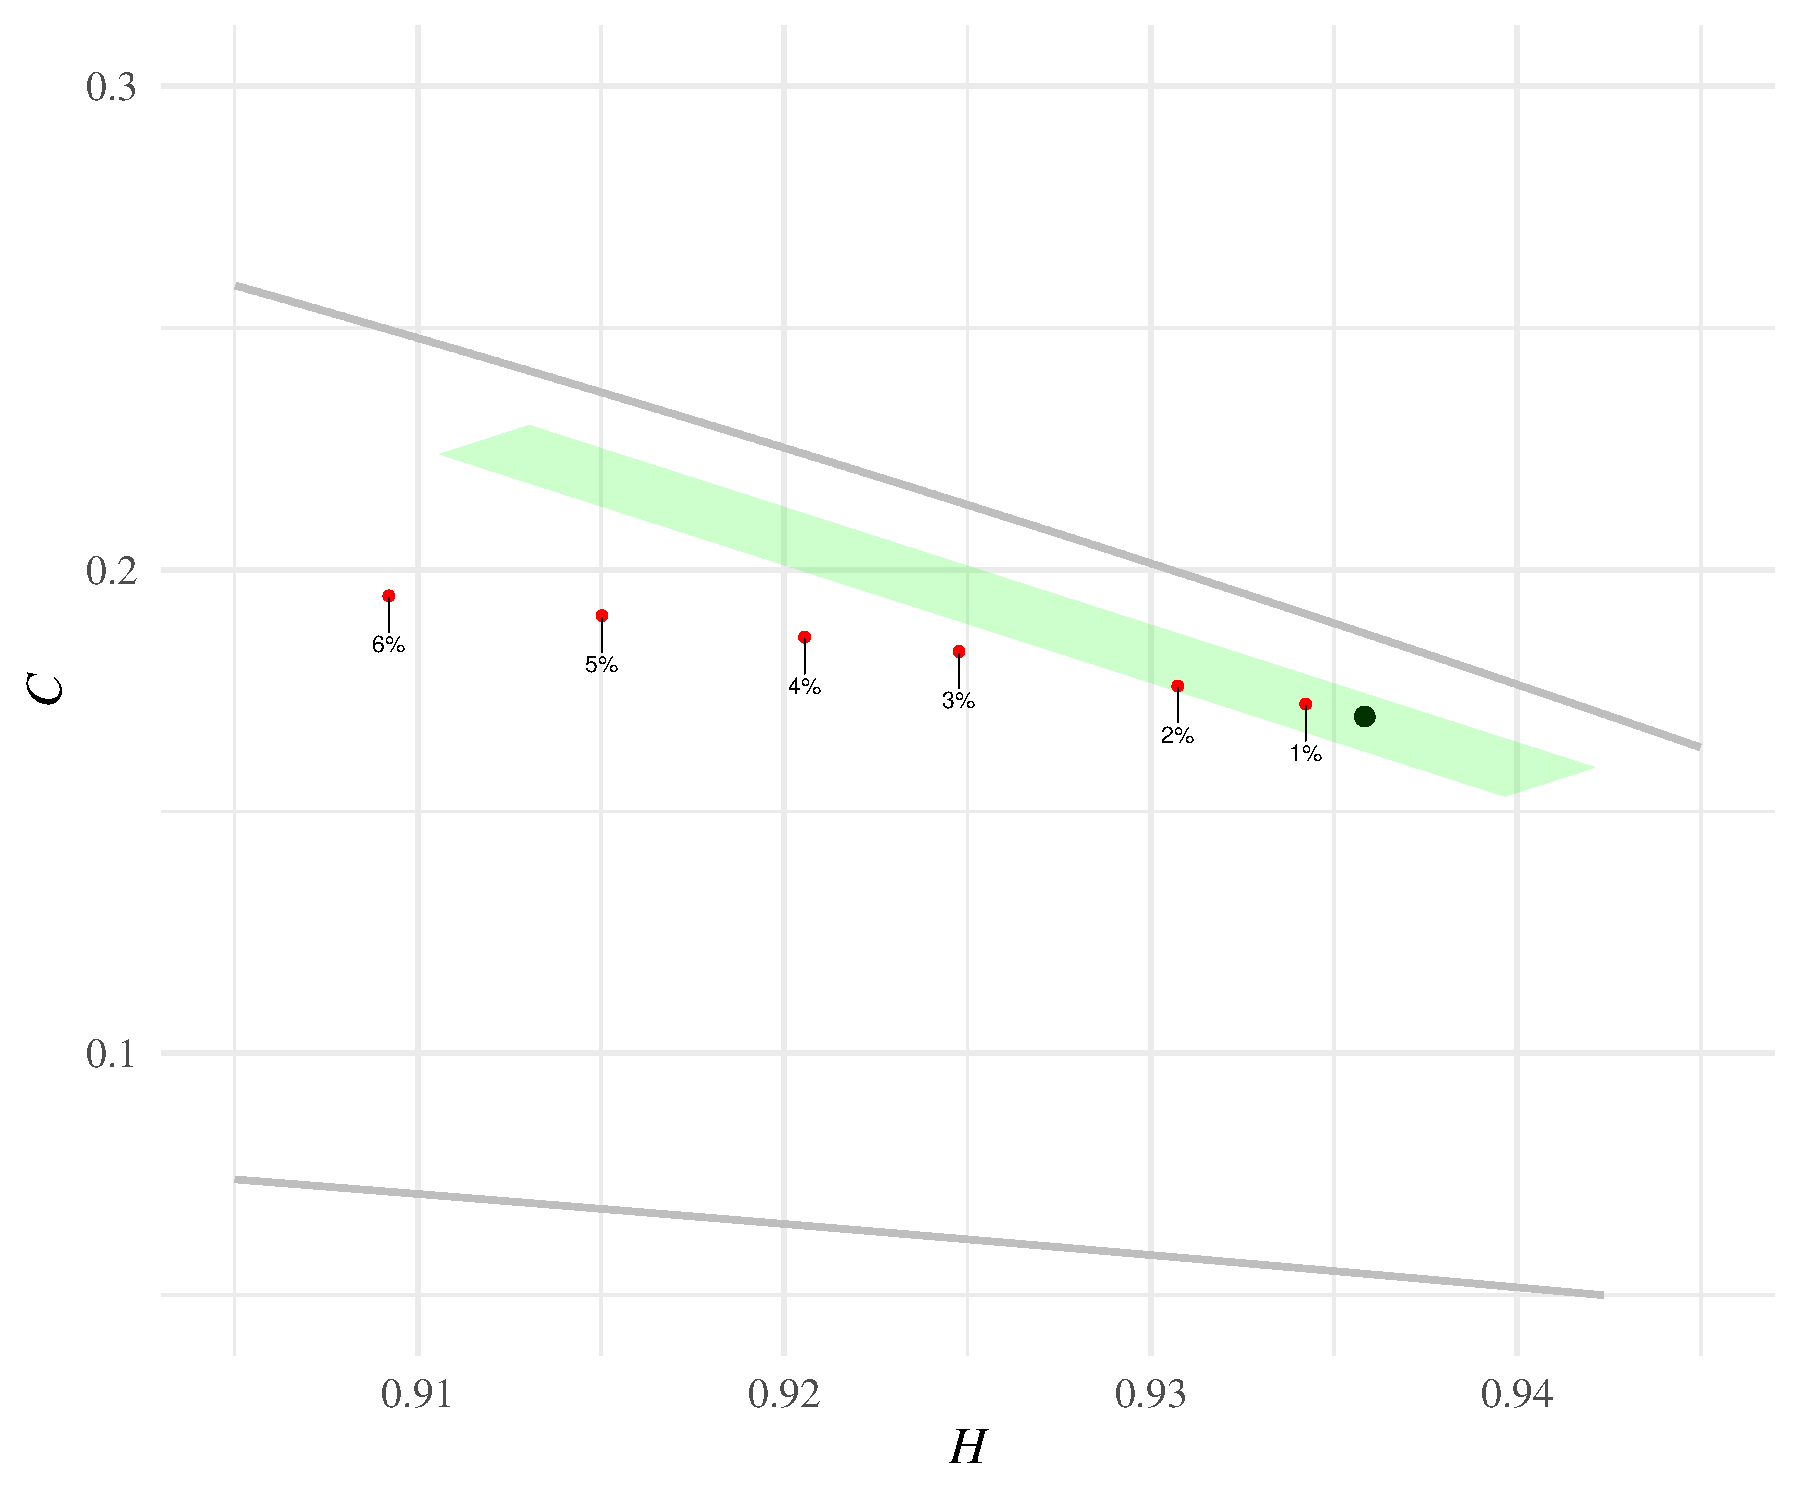
\includegraphics[width=.7\linewidth]{Figures/PointsPatchedIncreasingFunction}
		\caption{Effect of patching an increasing function at different levels to a white noise sequence.}\label{Fig:PointsPatchedIncreasingFunction}
	\end{figure}
	
	The original point is displaced, at all levels of contamination, to a region with smaller entropy and larger complexity.
	When the percentage of contamination is below approximately \SI{2}{\percent}, the test will not reject the null hypothesis at the \SI{99}{\percent}; in fact, the $p$-value is of around \SI{1.5}{\percent} for $c=0,0.01,0.02$.
	The $p$-value falls to orders of $10^{-6}$ when the contamination is of \SI{3}{\percent} and above. 
	
	It is worth noticing that a test based solely on the entropy would have less power.
	In this case, the complexity component enables the test to reject the null hypothesis at small contamination percentages.
\end{quote}



\section{Reviewer \#2}

\vskip3em\begin{tcolorbox}[colback=red!5!white,colframe=red!75!black,title=Comment \#1]
The paper address an interesting problem in time series. The manuscript presents a thorough review of the literature, and develops a proposed test for a wide array of models. Examples and simulation studies are clearly defined and their results are discussed. The paper is well written, and I have no major corrections to propose.
\end{tcolorbox}

Thank you very much for your encouraging comments.

\bibliography{References}

\end{document}

